\documentclass[english,floatsintext,man]{apa6}

\usepackage{amssymb,amsmath}
\usepackage{ifxetex,ifluatex}
\usepackage{fixltx2e} % provides \textsubscript
\ifnum 0\ifxetex 1\fi\ifluatex 1\fi=0 % if pdftex
  \usepackage[T1]{fontenc}
  \usepackage[utf8]{inputenc}
\else % if luatex or xelatex
  \ifxetex
    \usepackage{mathspec}
    \usepackage{xltxtra,xunicode}
  \else
    \usepackage{fontspec}
  \fi
  \defaultfontfeatures{Mapping=tex-text,Scale=MatchLowercase}
  \newcommand{\euro}{€}
\fi
% use upquote if available, for straight quotes in verbatim environments
\IfFileExists{upquote.sty}{\usepackage{upquote}}{}
% use microtype if available
\IfFileExists{microtype.sty}{\usepackage{microtype}}{}

% Table formatting
\usepackage{longtable, booktabs}
\usepackage{lscape}
% \usepackage[counterclockwise]{rotating}   % Landscape page setup for large tables
\usepackage{multirow}		% Table styling
\usepackage{tabularx}		% Control Column width
\usepackage[flushleft]{threeparttable}	% Allows for three part tables with a specified notes section
\usepackage{threeparttablex}            % Lets threeparttable work with longtable

% Create new environments so endfloat can handle them
% \newenvironment{ltable}
%   {\begin{landscape}\begin{center}\begin{threeparttable}}
%   {\end{threeparttable}\end{center}\end{landscape}}

\newenvironment{lltable}
  {\begin{landscape}\begin{center}\begin{ThreePartTable}}
  {\end{ThreePartTable}\end{center}\end{landscape}}




% The following enables adjusting longtable caption width to table width
% Solution found at http://golatex.de/longtable-mit-caption-so-breit-wie-die-tabelle-t15767.html
\makeatletter
\newcommand\LastLTentrywidth{1em}
\newlength\longtablewidth
\setlength{\longtablewidth}{1in}
\newcommand\getlongtablewidth{%
 \begingroup
  \ifcsname LT@\roman{LT@tables}\endcsname
  \global\longtablewidth=0pt
  \renewcommand\LT@entry[2]{\global\advance\longtablewidth by ##2\relax\gdef\LastLTentrywidth{##2}}%
  \@nameuse{LT@\roman{LT@tables}}%
  \fi
\endgroup}


  \usepackage{graphicx}
  \makeatletter
  \def\maxwidth{\ifdim\Gin@nat@width>\linewidth\linewidth\else\Gin@nat@width\fi}
  \def\maxheight{\ifdim\Gin@nat@height>\textheight\textheight\else\Gin@nat@height\fi}
  \makeatother
  % Scale images if necessary, so that they will not overflow the page
  % margins by default, and it is still possible to overwrite the defaults
  % using explicit options in \includegraphics[width, height, ...]{}
  \setkeys{Gin}{width=\maxwidth,height=\maxheight,keepaspectratio}
\ifxetex
  \usepackage[setpagesize=false, % page size defined by xetex
              unicode=false, % unicode breaks when used with xetex
              xetex]{hyperref}
\else
  \usepackage[unicode=true]{hyperref}
\fi
\hypersetup{breaklinks=true,
            pdfauthor={},
            pdftitle={Still suspicious: The suspicious coincidence effect revisited},
            colorlinks=true,
            citecolor=blue,
            urlcolor=blue,
            linkcolor=black,
            pdfborder={0 0 0}}
\urlstyle{same}  % don't use monospace font for urls

\setlength{\parindent}{0pt}
%\setlength{\parskip}{0pt plus 0pt minus 0pt}

\setlength{\emergencystretch}{3em}  % prevent overfull lines

\ifxetex
  \usepackage{polyglossia}
  \setmainlanguage{}
\else
  \usepackage[english]{babel}
\fi

% Manuscript styling
\captionsetup{font=singlespacing,justification=justified}
\usepackage{csquotes}
\usepackage{upgreek}



\usepackage{tikz} % Variable definition to generate author note

% fix for \tightlist problem in pandoc 1.14
\providecommand{\tightlist}{%
  \setlength{\itemsep}{0pt}\setlength{\parskip}{0pt}}

% Essential manuscript parts
  \title{Still suspicious: The suspicious coincidence effect revisited}

  \shorttitle{The suspicious coincidence effect revisited}


  \author{Molly L. Lewis\textsuperscript{1,2}~\& Michael C. Frank\textsuperscript{3}}

  \def\affdep{{"", ""}}%
  \def\affcity{{"", ""}}%

  \affiliation{
    \vspace{0.5cm}
          \textsuperscript{1} Computation Institute, University of Chicago\\
          \textsuperscript{2} Department of Psychology, University of Wisconsin, Madison\\
          \textsuperscript{3} Department of Psychology, Stanford University  }

 % If no author_note is defined give only author information if available
      \newcounter{author}
                              \authornote{
            Correspondence concerning this article should be addressed to Molly L. Lewis. E-mail: \href{mailto:mollylewis@uchicago.edu}{\nolinkurl{mollylewis@uchicago.edu}}
          }
                                  
  \note{\(^*\)To whom correspondence should be addressed. Email:
\href{mailto:mollylewis@uchicago.edu}{\nolinkurl{mollylewis@uchicago.edu}}}

  \abstract{Enter abstract here. Each new line herein must be indented, like this
line.}
  \keywords{word learning, Bayesian inference, meta-analysis, concepts \\

    \indent Word count: X
  }




  \usepackage{setspace}
  \usepackage{float}
  \usepackage{graphicx}
  \AtBeginEnvironment{tabular}{\singlespacing}
  \usepackage{pbox}
  \usepackage{hyphsubst}

\usepackage{amsthm}
\newtheorem{theorem}{Theorem}
\newtheorem{lemma}{Lemma}
\theoremstyle{definition}
\newtheorem{definition}{Definition}
\newtheorem{corollary}{Corollary}
\newtheorem{proposition}{Proposition}
\theoremstyle{definition}
\newtheorem{example}{Example}
\theoremstyle{remark}
\newtheorem*{remark}{Remark}
\begin{document}

\maketitle

\setcounter{secnumdepth}{0}



\subsection{Intro}\label{intro}

Suppose you're learning a foreign language and you learn that a chili
pepper can be called \enquote{wug.} What does \enquote{wug} mean? This
question is challenging of course because the same object can be refered
to by many different labels depending on the level of abstraction that
the speaker wishes to convey. One could refer to the same chili pepper
using the labels \enquote{chili pepper} at the subordinate level,
\enquote{pepper} at the basic level, or \enquote{vegetable} at the
superodinate level. For the naive learner, this ambiguity poses a
fundamental challenge for inferring the meaning of the word since every
instance of \enquote{wug} that the learner hears is consistent with
extensions at all three levels of abstraction. Furthermore, children
rarely receive the kind of negative evidence (\enquote{this is
\emph{not} a wug}) that would help disambiguate the word's meaning. Yet,
despite the apparent difficulty of the learning problem, children
sucessfully learn words at multiple levels of abstraction.

Xu and Tenenbaum (2007a; henceforth XT) provide one account as to how
children might learn such words without relying on negative evidence.
Within a Bayesian framwork, they suggest that learners implicitly
consider the likelihood of hearing different word-objects pairs under
different hypotheses about the extension of a word. One consequence of
this assumption is that learners should be sensitive to the number of
word-objects pairs they observe when determining a word's meaning. In
particular, XT predict that a learner should think that it would be a
\enquote{suspcious coincidence} to observe three subordinate examples
(e.g., chili peppers) with the word \enquote{wug} if the true meaning of
the word were at the basic level (e.g., pepper). More generally, they
predict that a learner should be more likely to generalize narrowly to
the subordinate level when they observe more word-object pairs. In two
experiments, they find that both adults and children show exactly this
pattern.

This finding has been foundational to a number of other more recent
findings. * strong sampling * Gweon, Tenenbaum, and Schulz (2009) {[}TO
DO{]}

In a follow-up study to XT, Spencer, Perone, Smith, and Samuelson (2011;
henceforth SPSS) offer an alternative explanation for the suspcicious
coincidence effect. They argue that the effect can be accounted for by
basic memory processes in which the co-occurence of objects in time and
space highlights differences across exemplars, thus leading to increased
conceptual discrimination. They predict that this increased conceptual
discrimination should make it more likely for participants to generalize
to the subordinate level when more subordinate category exemplars are
observed---the suspicious coincidence pattern observed by XT. SPSS test
this possibility by replicating the original XT experiments with one
small change: Rather than presenting the learning exemplars
simulateneously, they present them in sequence such that only one
learning exemplar is visible at a time. The sequential presentation of
objects, the argue, more closely reflects the experience of learners in
the real world who encounter objects in time and space.

In a series of experiments, SPSS replicate XT's finding with
simultaneous presentation of the learning exemplars, but fail to
replicate it with the sequential presentation. In fact, they observe a
reversal of the effect under sequential presentation conditions, such
that participants were more likely to generalize to the basic level when
more subordinate exemplars were presented.

These findings are surprising in part because it is not clear that
effects of basic memory processes should lead to broader generalization.
While SPSS argue that simultaneous presentation highlights differences
across exemplars, others have suggested that this method highlights
their commonalities and increases memory consolidation, thus predicting
\emph{greater} generalization in the sequential condition (Lawson,
2017). Indeed, several findings suggest that preschoolers demonstrate
the suspicious coinccendince effect when generalizing properties under
sequential presentation (Lawson, 2014), and that this effect disappears
under simultanous presentation (Lawson, 2017).

On the other hand, there is reason to think that estimates of rational
inference in word learning may be over-estimated. In other work, we find
that a related effect predicted by XT (Xu \& Tenenbaum, 2007a)---strong
versus weak sampling---appears to be much smaller in magnitude relative
to the original estimate (Lewis \& Frank, 2016).

Given the theoretical importance of the suspicious coincidence effect
and the conflicting empirical picture, we sought to replicate the
suspicious coincidence effect. We report 12 experiments, 10 of which
were pre-registered, that varied four design aspects that differed
between XT and SPPS: Presentation timing, trial order, blocking, and
label consistency. We recover the suspicious coincidence effect with a
large effect size in both sequential and simultaneous presentation
conditions. The effect only occurs, however, in experiments where the
trial with one exemplar is presented \emph{before} the key trial with
three subordinate-consistent exemplars (the \enquote{suspicious
coincidence}). We attribute this difference to participants' awareness
of the possibility of subordinate generalizations following the
three-exemplar trial; in these conditions, we see a high level of
subordinate generalizations even for the one-exemplar trial (leading to
the absence of a difference between conditions). In sum, and contra
SPSS, the \enquote{suspicious coincidence} effect is robust to
sequential presentation. The effect is sensitive to some features of the
general experimental context, however, suggesting a potential
interpretation in terms of the pragmatics of the task.

\section{Methods}\label{methods}

We report how we determined our sample size, all manipulations, and all
measures in the study. All stimuli, experimental code, sample sizes, and
analyses were pre-registered with the exception of Exps. 4 and 8, and
publically available (\url{https://osf.io/yekhj/}).

\subsection{Participants}\label{participants}

Fifty participants were recruited on Amazon Mechanical Turk for each of
our 12 experiments (N = 600), and paid 40-50 cents for their
participation. Across all 12 experiments, 13\% of participants completed
more than one experiment. We report data from all participants in the
Main Text, but the pattern of reported findings holds when these
participants are excluded (see
SI)\footnote{Supplemental information can be found at "}.

We determined our sample size on the basis of a pre-registered power
calculation using a meta-analytic estimate of the effect size from
studies conducted by XT and SPSS. The chosen sample size was
approximately twice the estimated sample size necessary to obtain a
power of 1.

\begin{figure}[t!]
 
 {\centering 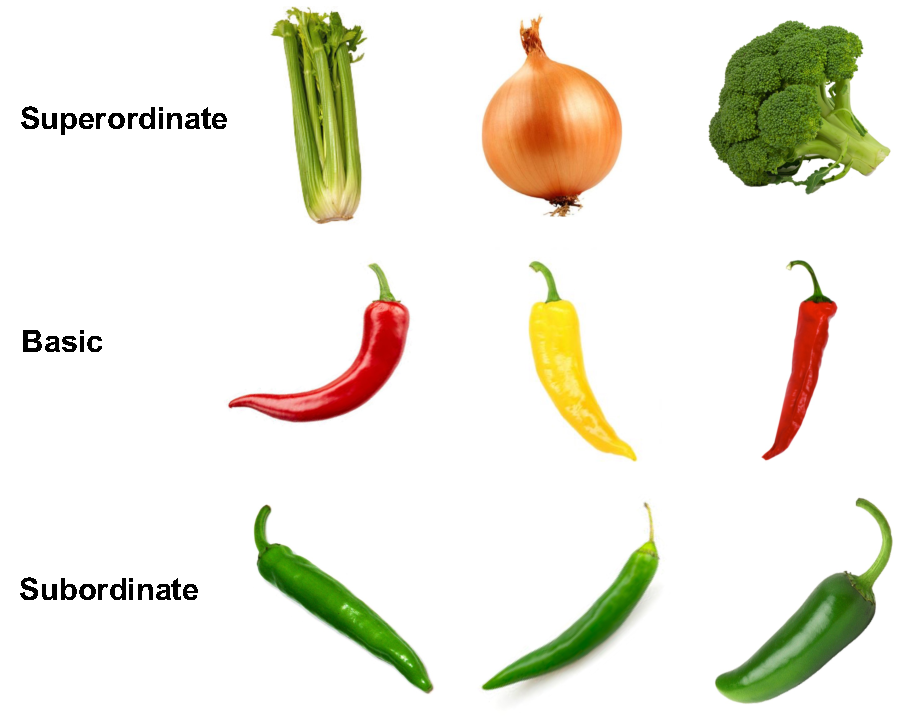
\includegraphics[width=0.5\linewidth]{figs/stim} 
 
 }
 
 \caption{Sample stimuli. Three superodinate (top), basic (middle), and subordinate (bottom) exemplars from the vegetable category.}\label{fig:unnamed-chunk-1}
 \end{figure}

\subsection{Stimuli}\label{stimuli}

Our stimuli closely replicated that of XT and SPSS. The linguistic
stimuli were 12 one-syllable novel labels (e.g., \enquote{wug}), and the
referent objects were three sets of 15 pictures from different basic
level categories (vegetables, vehicles and animals). Within each
category, five were subordinate exemplars (e.g.~green pepper), four were
basic level exemplars (e.g.~peppers), and six were superordinate
exemplars (e.g.~vegetables; Fig.~1). The exemplars were divided into a
learning and generalization set. For each category, the learning set
consisted of 3 subordinate, 2 basic, and 2 superordinate pictures
presented in different combinations on different trials (see Procedure).
The generalization set for each category consisted of the remaining 8
pictures. The learning and generalization sets were the same for all
participants.

\subsection{Procedure}\label{procedure}

\begin{table}

\caption{\label{tab:unnamed-chunk-2}Summary of our 12 experiments.}
\centering
\fontsize{12}{14}\selectfont
\begin{tabular}[t]{crrrrrrr}
\toprule
\multicolumn{2}{c}{ } & \multicolumn{4}{c}{Manipulations} & \multicolumn{1}{c}{ } \\
\cmidrule(l{2pt}r{2pt}){3-6}
Exp. & N & Timing & Order & Blocking & Label & Effect Size & Original 
Exp.\\
\midrule
1 & 50 & simult. & 1-3 & pseudo-random & same & 1.32 [1.24, 1.4] & XT E1/E2\\
2 & 50 & simult. & 1-3 & pseudo-random & same & 1.14 [1.06, 1.22] & XT E1/E2\\
3 & 50 & simult. & 1-3 & pseudo-random & diff. & 1.16 [1.08, 1.24] & \\
4 & 50 & seq. & 1-3 & pseudo-random & same & 1.42 [1.32, 1.52] & \\
5 & 50 & seq. & 1-3 & pseudo-random & diff. & 1.26 [1.18, 1.34] & \\
\addlinespace
6 & 50 & seq. & 1-3 & blocked & diff. & 1.31 [1.23, 1.39] & \\
7 & 50 & simult. & 3-1 & blocked & diff. & 0.02 [-0.06, 0.1] & SPSS ES1/ES2\\
8 & 50 & simult. & 3-1 & blocked & diff. & -0.06 [-0.14, 0.02] & \\
9 & 50 & simult. & 3-1 & blocked & same & -0.14 [-0.22, -0.06] & \\
10 & 50 & seq. & 3-1 & blocked & diff. & -0.44 [-0.52, -0.36] & SPSS E2/E3\\
\addlinespace
11 & 50 & seq. & 3-1 & pseudo-random & same & -0.31 [-0.39, -0.23] & \\
12 & 50 & seq. & 3-1 & blocked & same & -0.17 [-0.25, -0.09] & \\
\bottomrule
\multicolumn{8}{l}{\textsuperscript{1} N = sample size; Timing = presentation timing (sequential or simultaneous); Order =}\\
\multicolumn{8}{l}{relative ordering of 1 and 3 subordinate trials; Blocking = trials blocked by category or}\\
\multicolumn{8}{l}{pseudo-random; Label = same or different label in 1 and 3 trials; Effect size = Cohen's d}\\
\multicolumn{8}{l}{[95\% CI]; Original Exp. = corresponding experiment from prior literature.}\\
\end{tabular}
\end{table}

Participants were first introduced to a picture of a character
(\enquote{Mr.~Frog}) and instructions describing the task. They were
told that the character speaks a different language and their job was to
help the character find the toys he wants. Participants then advanced to
the main experiment, which consisted of a series of 12 trials on
separate screens. On each trial, one or three learning exemplars from
one of the three stimulus categories appeared at the top of the screen,
along with the following instructions: \enquote{Here {[}is a wug/are
three wugs{]}. Can you give Mr.~Frog all of the other wugs?.} Below the
learning exemplars, 24 generalization exemplars (8 from each of the 3
categories) were displayed in a 4\emph{x}6 grid. The order of
generalizaiton pictures was randomized across trials. Participants were
instructed to select the target category members (\enquote{To give a
wug, click on it below. When you have given all the wugs, click the Next
button.}). When an exemplar was selected, a red box appeared around the
picture, and participants were allowed to change their selections by
clicking on the picture a second time. The learning exemplars remained
visible at the top of the screen during the generalization task. Once
they had made their selections, participants advanced to the next trial
by clicking the \enquote{Next} button.

There were four trial types distinguished by the number and semantic
level of the learning exemplars: one subordinate exemplar, three
subordinate exemplars, three basic exemplars, and three superordate
exemplars. Each participant completed each trial type for each of the
three stimulus categories (vegetables, vehicles, and animals).

Across 12 experiments, we manipulated four aspects of the trial design
that differed between XT and SPSS (summarized in Table 1): Presentation
timing (simultaneous vs.~sequential), trial order (1-3 vs.~3-1), label
(same vs.~different), and blocking (blocked
vs.~pseudo-random)\footnote{All experiments can be viewed directly at XXX.}.
We describe each of these factors in more detail below.

\subsubsection{Presentation Timing}\label{presentation-timing}

Presentation timing was the key, theoretically motivated experimental
design difference between the XT (E1 and
E2\footnote{XT E1 and E2 differed in the age of participants (adults vs. children), but we collapse across this difference for the present analyses.})
and SPSS (E2 and E3). In XT, the learning exemplars were presented
statically and simultaneously, while in SPSS, participants saw a
sequence of individual exemplars with each exemplar visible only for 1s
at a time. In the sequential design, three exemplar learning trials
displayed pictures at three different locations (left, middle, and
right) in a sequence that repeated twice, for a total of 6s.

We reproduced these design aspects in the simultaneous and sequential
versions of our experiments. In the single exemplar, sequential trials,
the exemplar appeared (1s) and disappeared (1s) for three repetitions.
The generalization pictures did not appear in the sequential condition
until after the training pictures has appeared for 6 seconds, but
remained visibile as participants selected generalization exemplars.

\subsubsection{Trial order}\label{trial-order}

In XT, the three one-subordinate trials occured first followed by all
other trial types. In contrast, in SPSS (E2 and E3), the
three-subordinate trials occured first. SPSS's replication of XT's
simultanous design (SPSS E1) used the 1-3 ordering.{[}This isn't
actually quite true: \enquote{The first block of trials always involved
either one exemplar or three subordinate-level exemplars from each
domain. The remaining blocks of trials were randomly ordered for each
participant}\ldots{} so 1 exemplar trials were first only half the
time?{]}.

\subsubsection{Labels}\label{labels}

XT used the same label for each category for the three-subordinate and
one-suborinate trials. SPSS used a different novel label on each of the
12 trials, such that the three-subordinate and one-subordinate trials
were refered to with distinct labels. We reproduced these two design
choices, and also randomized labels across trials.

\subsubsection{Blocking}\label{blocking}

Finally, the studies by XT and SPSS differ in terms of whether the
trials were blocked by trial type: In XT, the first three trials were a
block of one-subordinate trials and the remaining 9 trials were
randomized, whereas SPSS blocked all four trial types. We also
reproduced these designs, randomizing within each block.

\subsection{Data analysis}\label{data-analysis}

The key prediction of the suspicious coincidence effect is that
participants should generalize to the basic level more often in
one-subordinate trials relative to three-subordinate trials. To measure
this, for each trial, we calculated the proportion generalizations to
subordinate exemplars within the same category (out of 2) and basic
exemplars within the same category (out of 2), and averaged across
categories for each participant. We estimated the difference between the
one-subordinate and three-subordinate conditions by calculating an
effect size (Cohen's \emph{d}) for each experiment. We then estimated
the influence of each our design manipulations on the overall effect
size by fitting a random-effect meta-analytic model with each of our
four manipulations as fixed effects. We used the metafor package
(Viechtbauer, 2010) in R to fit our meta-analytic models.

\section{Results}\label{results}

\begin{figure}
\centering
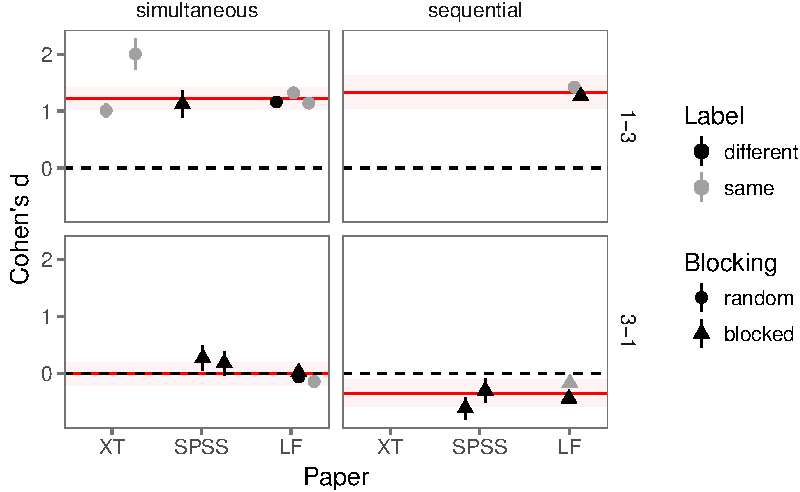
\includegraphics{xtmem_files/figure-latex/unnamed-chunk-3-1.pdf}
\caption{\label{fig:unnamed-chunk-3}Mean proportion generalizations to basic
level exemplars in the one (pink) and three (green) subordinate exemplar
conditions for all 12 of our experiments. Each facet corresponds to a
pairing of presentation timing (simultaneous vs.~sequential) and trial
order (1-3 vs.~3-1). Error bars are bootstrapped 95\% confidence
intervals.}
\end{figure}

Figure \ref{fig:means_fig}shows the mean proportion generalizations to
the basic level in the one- and three-subordinate trials for all 12
experiments\footnote{See SI for means across all measures and conditions},
and Figure \ref{fig:effect_sizes_fig} shows the corresponding effect
sizes (with XT and SPSS experiments included for reference).

\begin{figure}
\centering
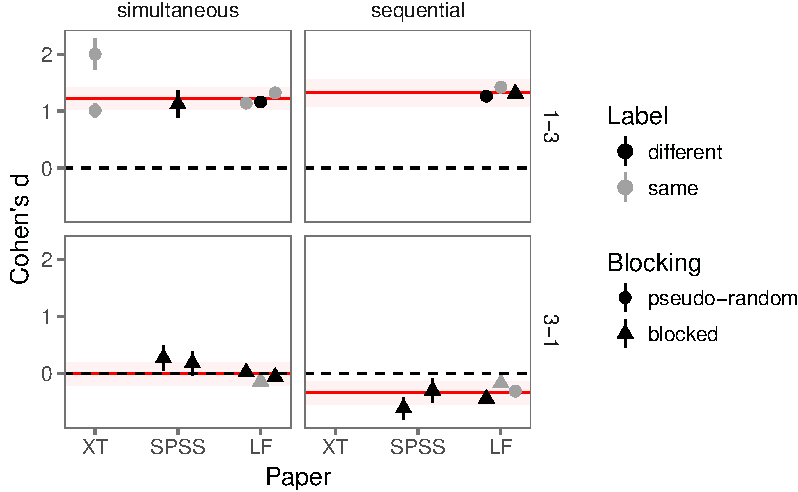
\includegraphics{xtmem_files/figure-latex/unnamed-chunk-4-1.pdf}
\caption{\label{fig:unnamed-chunk-4}Effect sizes for all 19 studies
conducted on the suspicious coincidence effect by XT (Xu \& Tenenbaum,
2007a), SPSS (Spencer, et al, 2011), and the current authors. The
top-bottoom facets indicate whether the single exemplar trial occurred
first (1-3) or second (3-1). The left-right facets indicate whether the
exemplars were presented simulateously as in XT or sequentially as in
SPSS. Point color indicates whether the single exemplar and three
subordinate exemplars received the same (grey) or different (black)
label. Point shape indicates whether trials were blocked by category
(circle) or pseudo-random (triangle). Points are jittered along the
x-axis for visibility. The red line reflects the meta-analytic estimate
of the effect size (for the XT experiments, standard deviations on
effect sizes are estimated from the SPSS replication). All error bars
are 95\% confidence intervals.}
\end{figure}

In two exact replications of the XT method (XT E1 and X2), we replicate
the suspicious coincidence effect (Exp. 1: \emph{d} = 1.32 {[}1.24,
1.4{]}; Exp. 2: \emph{d} = 1.14 {[}1.06, 1.22{]}), with a magnitude
comparable to the original XT experiments (\emph{d} = 2 {[}1.73, 2.27{]}
and \emph{d} = 1.01 {[}0.89, 1.13{]}). We also replicate the reversal in
the suspicious coincidence effect observed by SPSS (SPSS E2 and E3) in
an exact replication of their method (Exp. 10; \emph{d} = -0.44
{[}-0.52, -0.36{]}), and with a magnitude comparable to the original
experiments (SPSS E2: \emph{d} = -0.61 {[}-0.81, -0.41{]}; SPSS E3:
\emph{d} = -0.3 {[}-0.52, -0.08{]}).

\begin{table}

\caption{\label{tab:unnamed-chunk-5}Meta-analytic model with manipulations as fixed effects.}
\centering
\fontsize{12}{14}\selectfont
\begin{tabular}[t]{lrrr}
\toprule
Fixed effect & beta & z-value & p-value\\
\midrule
Intercept & 1.37 [1.09, 1.65] & 9.48 & <.0001\\
Simultaneous vs. sequential timing & -0.13 [-0.33, 0.08] & -1.18 & 0.24\\
1-3 vs. 3-1 trial order & -1.48 [-1.77, -1.18] & -9.90 & <.0001\\
Different vs. same label & 0.03 [-0.21, 0.26] & 0.20 & 0.84\\
Blocked vs. pseudo-random trial structure & -0.09 [-0.41, 0.24] & -0.52 & 0.6\\
\bottomrule
\end{tabular}
\end{table}

Critically, however, the meta-analyic model across all 12 experiments
reveals that only trial order is a reliable predictor of effect size
(\(\beta\) = -1.48; \emph{Z} = -9.9; \emph{p} \textless{}.0001), while
timing (\(\beta\) = -0.13; \emph{Z} = -1.18; \emph{p} = 0.24), blocking
(\(\beta\) = -0.09; \emph{Z} = -0.52; \emph{p} = 0.6), and label are not
(\(\beta\) = 0.03; \emph{Z} = 0.2; \emph{p} = 0.84); Table 2). Contra
SPSS, this suggests that the suspcious coincidence is robust to
spatio-temoral aspects of the presentation learning exemplars. In the
General Discussion, we consider why trial order might influence the
suspicious coincidence effect.

\section{Discussion}\label{discussion}

\begin{itemize}
\tightlist
\item
  why is there a reversal: 1- 3 story
\item
  other task context effect: Lawson and Fischer (exp. 2), Lewis and
  Frank
\end{itemize}

\newpage

\section{References}\label{references}

\begin{center}\rule{0.5\linewidth}{\linethickness}\end{center}

nocite: \textbar{} Spencer, Perone, Smith, and Samuelson (2011) Xu and
Tenenbaum (2007b)

\setlength{\parindent}{-0.5in} \setlength{\leftskip}{0.5in}

\hypertarget{refs}{}
\hypertarget{ref-lawson2014three}{}
Lawson, C. A. (2014). Three-year-olds obey the sample size principle of
induction: The influence of evidence presentation and sample size
disparity on young children's generalizations. \emph{Journal of
Experimental Child Psychology}, \emph{123}, 147--154.

\hypertarget{ref-lawson2017influence}{}
Lawson, C. A. (2017). The influence of task dynamics on inductive
generalizations: How sequential and simultaneous presentation of
evidence impact the strength and scope of property projections.
\emph{Journal of Cognition and Development}.

\hypertarget{ref-lewis2016understanding}{}
Lewis, M. L., \& Frank, M. C. (2016). Understanding the effect of social
context on learning: A replication of xu and tenenbaum (2007b).
\emph{Journal of Experimental Psychology: General}, \emph{145}(9),
e72--e80.

\hypertarget{ref-spencer2011learning}{}
Spencer, J. P., Perone, S., Smith, L. B., \& Samuelson, L. K. (2011).
Learning words in space and time: Probing the mechanisms behind the
suspicious-coincidence effect. \emph{Psychological Science},
\emph{22}(8), 1049--1057.

\hypertarget{ref-R-metafor}{}
Viechtbauer, W. (2010). Conducting meta-analyses in R with the metafor
package. \emph{Journal of Statistical Software}, \emph{36}(3), 1--48.
Retrieved from \url{http://www.jstatsoft.org/v36/i03/}

\hypertarget{ref-xu2007}{}
Xu, F., \& Tenenbaum, J. B. (2007a). Sensitivity to sampling in Bayesian
word learning. \emph{Developmental Science}, \emph{10}(3), 288--297.

\hypertarget{ref-xu2007word}{}
Xu, F., \& Tenenbaum, J. B. (2007b). Word learning as Bayesian
inference. \emph{Psychological Review}, \emph{114}(2), 245.






\end{document}
